\documentclass[SE,authoryear,toc]{lsstdoc}
% lsstdoc documentation: https://lsst-texmf.lsst.io/lsstdoc.html
\input{meta}

% Package imports go here.
\usepackage{caption}
\usepackage{subcaption}

% Local commands go here.

%If you want glossaries
%\input{aglossary.tex}
%\makeglossaries

\title{Stuttered Image Analysis}

% Optional subtitle
% \setDocSubtitle{A subtitle}

\author{%
HyeYun Park, Claire-Alice Hebert, Craig Lage, Elana Urbach
}

\setDocRef{SITCOMTN-039}
\setDocUpstreamLocation{\url{https://github.com/lsst-sitcom/sitcomtn-039}}

\date{\vcsDate}

% Optional: name of the document's curator
% \setDocCurator{The Curator of this Document}

\setDocAbstract{%
We measure the centroids, PSFs, and ellipticity of the sources in stuttered images on AuxTel.
}

% Change history defined here.
% Order: oldest first.
% Fields: VERSION, DATE, DESCRIPTION, OWNER NAME.
% See LPM-51 for version number policy.
\setDocChangeRecord{%
  \addtohist{1}{YYYY-MM-DD}{Unreleased.}{HyeYun Park}
}


\begin{document}

% Create the title page.
\maketitle
% Frequently for a technote we do not want a title page  uncomment this to remove the title page and changelog.
% use \mkshorttitle to remove the extra pages

% ADD CONTENT HERE
% You can also use the \input command to include several content files.

\section{Introduction to Stuttered Images}

Readout of the AuxTel and LSSTCam CCDs occurs at about 0.5 Hz. To detect higher frequency contributions to seeing,
we take stuttered images. In these images:

\begin{enumerate}
  \item A bright star or double star pair is placed near the center of the CCD, but just offset enough so that it is on one amplifier.
  \item The shutter is opened.
  \item The CCD is exposed for a short period of time (generally 0.1 to 1 second).
  \item The CCD shifts some number of rows (generally 40 rows). The data from these rows is thrown away.
  \item Steps 3 and 4 are repeated until the CCD has fully shifted 2000 rows.
  \item The shutter is closed.
  \item The CCD is read out.
\end{enumerate}

\section{Data}

We take images on AuxTel both with bright single stars and with double stars of similar brightness with various displacements (see Fig.~\ref{fig:images}).

\begin{figure}[h]
\centering
\begin{subfigure}{.5\textwidth}
  \centering
  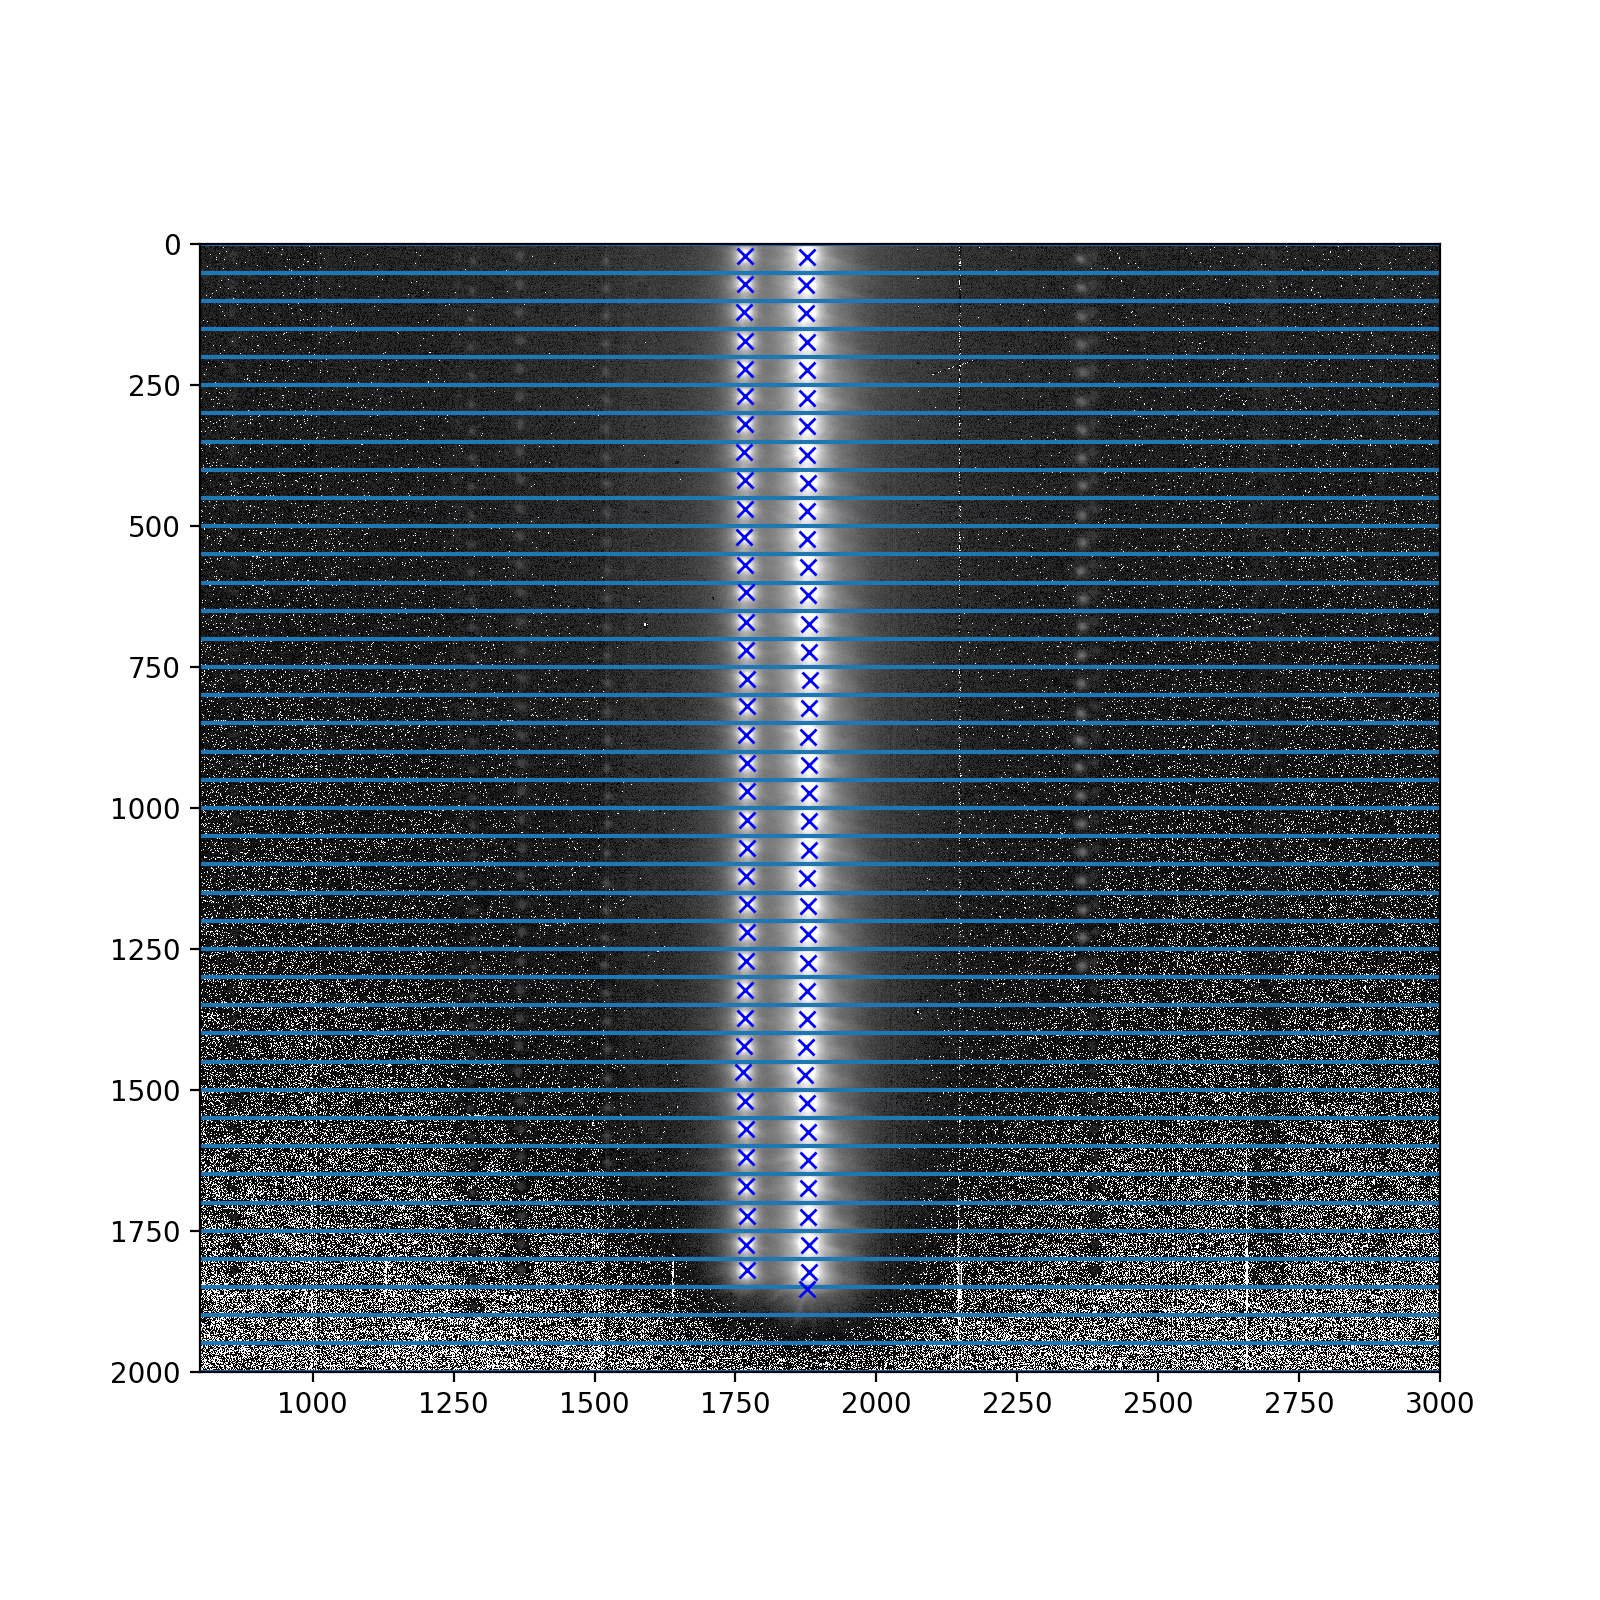
\includegraphics[width=1\linewidth]{20221012_close.png}
  \caption{}
  \label{fig:close}
\end{subfigure}%
\begin{subfigure}{.5\textwidth}
  \centering
  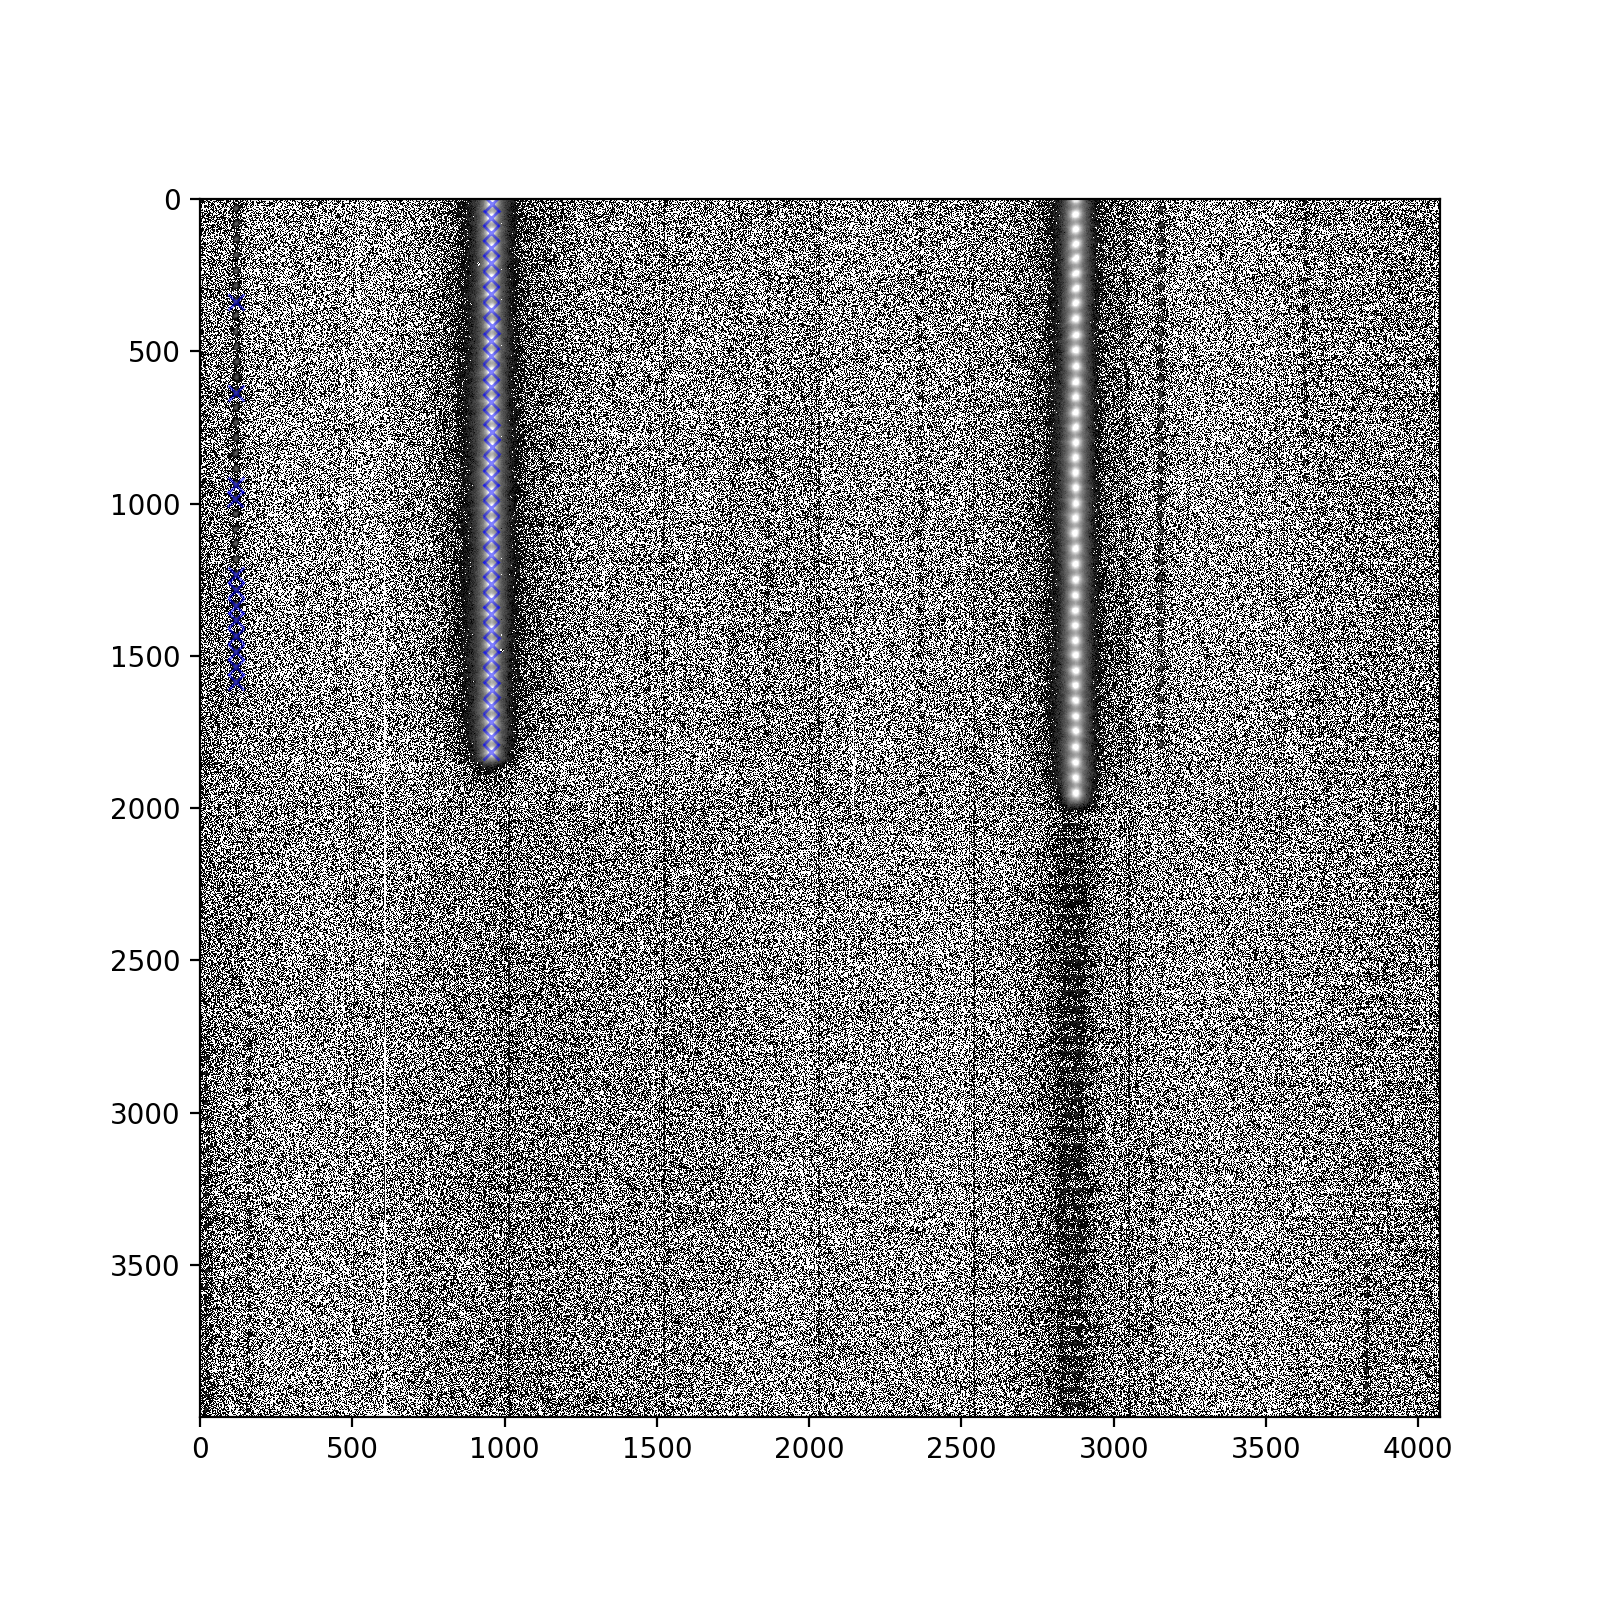
\includegraphics[width=1\linewidth]{20221012_far.png}
  \caption{}
  \label{fig:far}
\end{subfigure}
\caption{Double star images taken for stars that are (a) 12 arcsec (b) 180 (?) arcsec apart.}
\label{fig:images}
\end{figure}

\section{Analysis and Results}

\section{Conclusion}

\appendix
% Include all the relevant bib files.
% https://lsst-texmf.lsst.io/lsstdoc.html#bibliographies
\section{References} \label{sec:bib}
\renewcommand{\refname}{} % Suppress default Bibliography section
\bibliography{local,lsst,lsst-dm,refs_ads,refs,books}

% Make sure lsst-texmf/bin/generateAcronyms.py is in your path
\section{Acronyms} \label{sec:acronyms}
\addtocounter{table}{-1}
\begin{longtable}{p{0.145\textwidth}p{0.8\textwidth}}\hline
\textbf{Acronym} & \textbf{Description}  \\\hline

DM & Data Management \\\hline
\end{longtable}

% If you want glossary uncomment below -- comment out the two lines above
%\printglossaries





\end{document}
